% Options for packages loaded elsewhere
\PassOptionsToPackage{unicode}{hyperref}
\PassOptionsToPackage{hyphens}{url}
%
\documentclass[
]{article}
\usepackage{lmodern}
\usepackage{amssymb,amsmath}
\usepackage{ifxetex,ifluatex}
\ifnum 0\ifxetex 1\fi\ifluatex 1\fi=0 % if pdftex
  \usepackage[T1]{fontenc}
  \usepackage[utf8]{inputenc}
  \usepackage{textcomp} % provide euro and other symbols
\else % if luatex or xetex
  \usepackage{unicode-math}
  \defaultfontfeatures{Scale=MatchLowercase}
  \defaultfontfeatures[\rmfamily]{Ligatures=TeX,Scale=1}
\fi
% Use upquote if available, for straight quotes in verbatim environments
\IfFileExists{upquote.sty}{\usepackage{upquote}}{}
\IfFileExists{microtype.sty}{% use microtype if available
  \usepackage[]{microtype}
  \UseMicrotypeSet[protrusion]{basicmath} % disable protrusion for tt fonts
}{}
\makeatletter
\@ifundefined{KOMAClassName}{% if non-KOMA class
  \IfFileExists{parskip.sty}{%
    \usepackage{parskip}
  }{% else
    \setlength{\parindent}{0pt}
    \setlength{\parskip}{6pt plus 2pt minus 1pt}}
}{% if KOMA class
  \KOMAoptions{parskip=half}}
\makeatother
\usepackage{xcolor}
\IfFileExists{xurl.sty}{\usepackage{xurl}}{} % add URL line breaks if available
\IfFileExists{bookmark.sty}{\usepackage{bookmark}}{\usepackage{hyperref}}
\hypersetup{
  pdftitle={PNEUMONIC PLAGUE OUTBREAK IN NORTHEAST INDIA},
  pdfauthor={Zenabu, Zinhle, and Joseph},
  hidelinks,
  pdfcreator={LaTeX via pandoc}}
\urlstyle{same} % disable monospaced font for URLs
\usepackage[margin=1in]{geometry}
\usepackage{graphicx,grffile}
\makeatletter
\def\maxwidth{\ifdim\Gin@nat@width>\linewidth\linewidth\else\Gin@nat@width\fi}
\def\maxheight{\ifdim\Gin@nat@height>\textheight\textheight\else\Gin@nat@height\fi}
\makeatother
% Scale images if necessary, so that they will not overflow the page
% margins by default, and it is still possible to overwrite the defaults
% using explicit options in \includegraphics[width, height, ...]{}
\setkeys{Gin}{width=\maxwidth,height=\maxheight,keepaspectratio}
% Set default figure placement to htbp
\makeatletter
\def\fps@figure{htbp}
\makeatother
\setlength{\emergencystretch}{3em} % prevent overfull lines
\providecommand{\tightlist}{%
  \setlength{\itemsep}{0pt}\setlength{\parskip}{0pt}}
\setcounter{secnumdepth}{-\maxdimen} % remove section numbering
\usepackage{booktabs}
\usepackage{longtable}
\usepackage{array}
\usepackage{multirow}
\usepackage{wrapfig}
\usepackage{float}
\usepackage{colortbl}
\usepackage{pdflscape}
\usepackage{tabu}
\usepackage{threeparttable}
\usepackage{threeparttablex}
\usepackage[normalem]{ulem}
\usepackage{makecell}
\usepackage{xcolor}

\title{PNEUMONIC PLAGUE OUTBREAK IN NORTHEAST INDIA}
\author{Zenabu, Zinhle, and Joseph}
\date{17/01/2020}

\begin{document}
\maketitle

{
\setcounter{tocdepth}{2}
\tableofcontents
}
\newpage

\begin{figure}
\centering
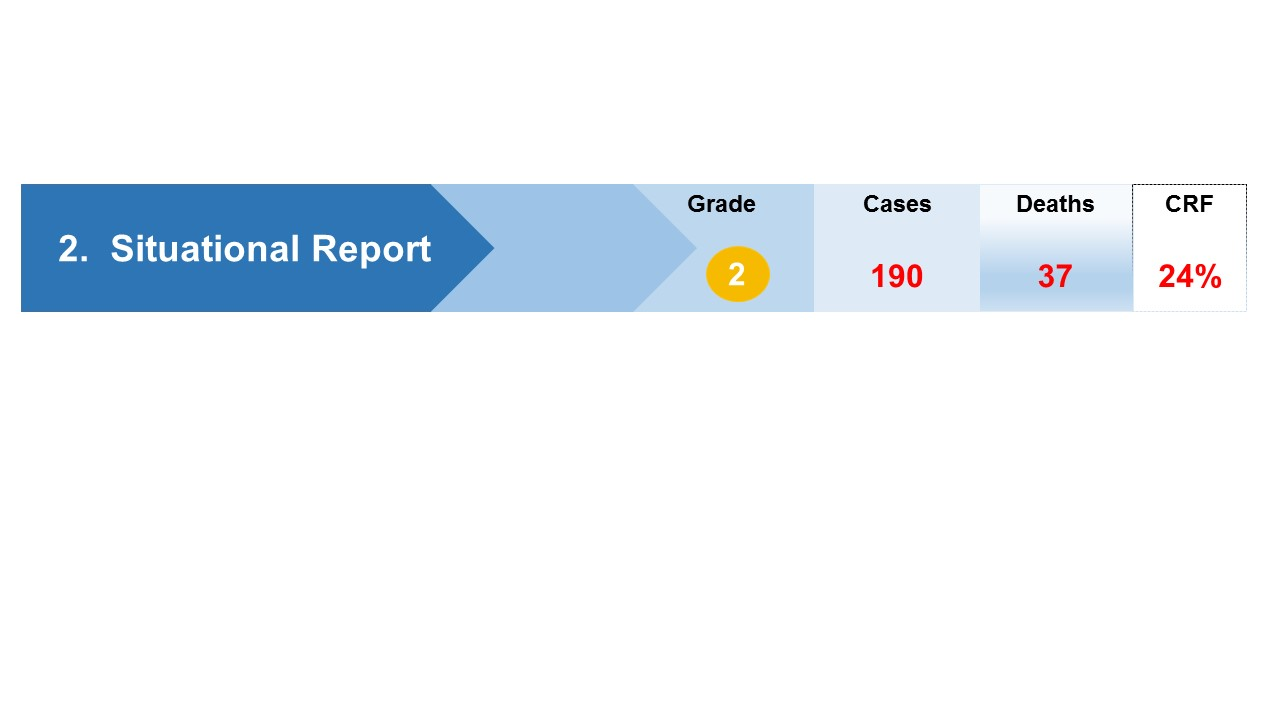
\includegraphics{~/GitHub/OutbreakResponse/resources/arrow_image.jpg}
\caption{Alt text}
\end{figure}

\hypertarget{background}{%
\section{Background}\label{background}}

Plague is a zoonotic disease caused by a bacteria found in rodents (1).
Individuals who are infected with plague usually manifest symptoms after
an incubation period of three to seven days. There are three main forms
of the plague disease: bubonic, septicaemic and pneumonic (2).
Transmission of the plague infection is through bites of an infected
rodent or inhalation of infected human respiratory droplets (1). It was
once a dreaded disease in India and claimed nearly 13 000 000 lives
between the years 1898 and 1994 (2,3). This disease has occurred in
India since the sixteenth century(2).

\hypertarget{case-definition}{%
\section{Case definition}\label{case-definition}}

Plague diagnosis is confirmed by laboratory diagnosis which can either
be by the isolation of Y. pestis from a clinical specimen or a
significant (fourfold or more) change in paired serum antibody titer to
\emph{Y. pestis} F1 antigen (4).

\hypertarget{symptoms}{%
\section{Symptoms}\label{symptoms}}

Symptoms of pneumonic plague include fever, headache, development of
pneumonia within a short space of time, followed by shortness of breath,
chest pain and cough. The patient may progress to respiratory failure
and shock if not treated within 2 to 4 days. If not treated, pneumonic
plague can be fatal (5).

\hypertarget{prevention}{%
\section{Prevention}\label{prevention}}

Currently, there is no vaccine for plague. People who came into direct
contact with infectious people must take antibiotics for seven days to
decrease chances of being infected (5). Patients who suspect they might
be infected with plague must wear surgical masks to prevent spreading
the diseases. Plague is usually caused by rodents and fleas, as part of
prevention, people are encouraged to reduce rodent habitats around them
and to keep fleas off their pets (6).

\hypertarget{situation-update}{%
\section{Situation update}\label{situation-update}}

We report on the progression of the recent pneumonic plague outbreak in
a community in northeast India which commenced on 12 October 2019. The
community has a population of 302 people. Between the 12th of October
2019 and 29th of November 2019, there were 189 reported cases, 160
confirmed cases and 29 probable cases. The outbreak has caused 24 deaths
to date.

The first case of the plague outbreak of India was detected on 11-Oct-19
and reached it's peak on 6-Nov-19. Majority 85\% out of 189 plague cases
were Lab confirmed.

\begin{flushleft}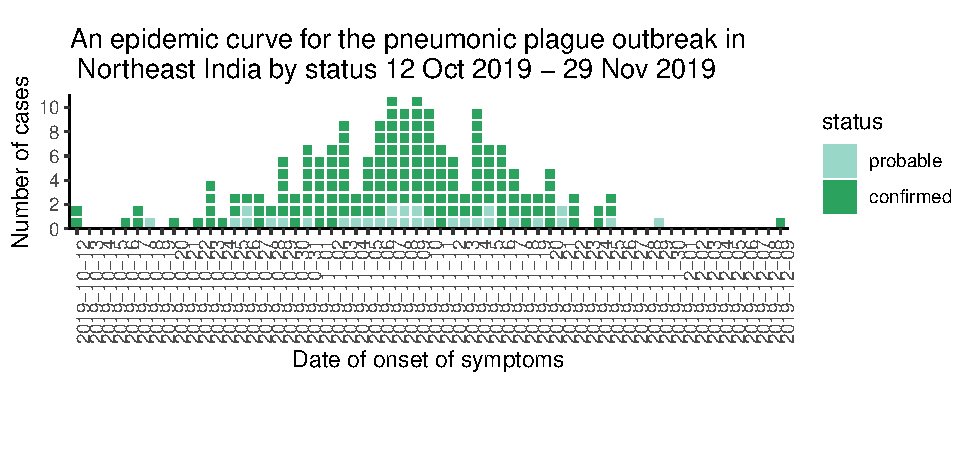
\includegraphics{Plague_SitRep_files/figure-latex/unnamed-chunk-2-1} \end{flushleft}

Of the 190 cases, majority 56.32\% were female. The first 3 cases of the
plague occured in females (Figure above) and it was five days later on
the 17-October 2019 when the first case was recored in the males.

\begin{flushleft}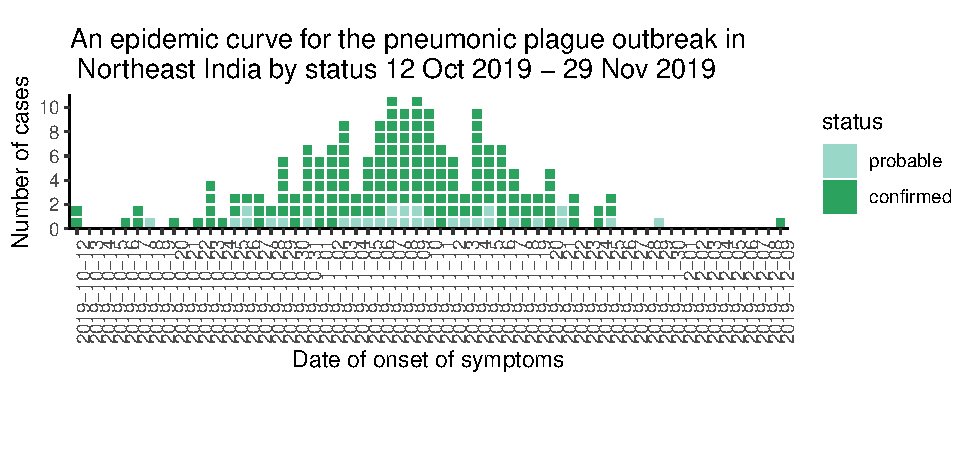
\includegraphics{Plague_SitRep_files/figure-latex/unnamed-chunk-3-1} \end{flushleft}

\hypertarget{data-needs}{%
\section{Data needs}\label{data-needs}}

We need genomic data on confirmed cases to study transmission patterns
in the dataset and GIS data to study the geographical distribution of
the cases in Himachal Pradesh, India.

\hypertarget{references}{%
\section{References}\label{references}}

\textbf{1} World Health Organization (WHO). Plague
\url{https://www.who.int/news-room/fact-sheets/detail/plague}
{[}accessed: 17 January 2020{]}

\textbf{2} World Health Organization (WHO). Plague Outbreak in
Madagascar.
\url{https://apps.who.int/iris/bitstream/handle/10665/259208/Ex-PlagueMadagascar0992017.pdf?sequence=2}
{[}accessed: 17 January 2020{]}

\textbf{3} Epidemiological studies of plague in India.
\url{https://www.ncbi.nlm.nih.gov/pmc/articles/PMC2555600/pdf/bullwho00328-0149.pdf}
{[}accessed: 17 January 2020{]}

\textbf{4} Centers for Disease Control and Prevention. (2020). Plague
(Yersinia pestis).
\url{https://wwwn.cdc.gov/nndss/conditions/plague/case-definition/2020/}
{[}accessed: 17 January 2020{]}

\textbf{5} Centers for Disease Control and Prevention. (4 April 2018).
Facts about pneumonic plague.
\url{https://emergency.cdc.gov/agent/plague/factsheet.asp} {[} accessed:
17 january 2020{]}

\textbf{6} Centers for Disease Control and Prevention. (27 November
2018). Plague: prevention.
\url{https://www.cdc.gov/plague/prevention/index.html} {[}accessed: 17
January 2020{]}

\end{document}
